\refstepcounter{section}
\section*{Lecture 08: Let the Force be with you!}
\addcontentsline{toc}{section}{Lecture 08: Let the Force be with you!}
From our previous definition of the 4-momentum, we can now define the 4-force as its derivative with respect to proper time. The 4-force is generally denoted by $\vb{\bar{K}}$. Thus,
$$ \fvec{K}:= \dv{\vb{\bar{p}}}{\tau} $$
Now, if we consider another frame, then we have:
$$\fvec{K}' = \dv{\fvec{p}'}{\tau'} = \dv{\tau}{\tau'}\dv{\qty(\Lambda \fvec{p})}{\tau}=1 \times \Lambda \dv{\fvec{p}}{\tau}=\Lambda \fvec{K}$$
This follows the rule of vector transformation and is thus a 4-vector. Moreover, note that, if $\fvec{K} =0$ then $\fvec{p}$ is conserved. So, in the relativisitc case too, \textit{momentum is conserved in absence of force}. 
\subsection{Emergence of Energy}
Note that when defining the 4-momentum, we obtained:
$$\fvec{p} = \gamma \qty(m_o c, m_o \tvec{v})$$
While the spatial components do have a clear Newtonian limit in case of $v<< c (\gamma\rightarrow 1)$, it is not apriori clear what $p^0 = \gamma m_o c$ represent. Let us try to find out in the limit $v<<c$!
\begin{align*}
    p^0 &= \frac{m_o c}{\sqrt{1-\sfrac{v^2}{c^2}}}\\
    &= m_oc \qty(1- \sfrac{v^2}{c^2})^{-\sfrac{1}{2}}\\
    &= m_o c\qty[1 + \frac{v^2}{2c^2}+ \SO\qty(\sfrac{v^4}{c^4})] \qquad (\text{from Taylor expansion})\\
\end{align*}
From the above thing, we obtain:
$$p^0 c = m_o c + \frac{1}{2}m_ov^2 + \SO\qty(\sfrac{v^4}{c^4})$$
The second term clearly resembles our familiar kinetic energy while we do not have a clear idea about the first term and the higher order terms. However, this quantity $p^0 c$ seems to be a right fit to be called the \textit{energy} (since it \textit{does}) contain one of the familiar energies. Let us then define the total energy of a relativistic particle as:
$$E:= p^0c$$
Earlier we had seen that the norm $\norm{\fvec{p}} = - m_o^2 c^2$. Using this we have:
\begin{alignat*}{3}
   &\qquad\qquad \fvec{p}\cdot\fvec{p}&&=-m_o^2c^2\\
    \implies& \gmn p^\mu p^\nu &&= -m_o^2c^2\\
    \implies & -(p^0)^2 + \norm{ \tvec{p}}^2 &&= -m_o^2c^2\\
    \implies & -\sfrac{E^2}{c^2} +\norm{ \tvec{p}}^2 &&= -m_o^2c^2\\
    \implies & m_o^2c^4 + \norm{ \tvec{p}}^2 c^2 &&=  E^2  \\
    \implies &\sqrt{m_o^2c^4 + \norm{ \tvec{p}}^2 c^2} &&=E  \qquad\qquad (\text{ignoring negative solution})
\end{alignat*}
In the rest frame of the particle, the 3-momentum vanish, and hence we get the celebrated: 
$$E = m_oc^2$$
Since the total energy of the particle $E = \sqrt{m_o^2c^4 + \norm{ \tvec{p}}^2 c^2}$, the kinetic energy can be obtained by subtracting the \textit{rest energy term}, that is, $\mathrm{K.E} = E-m_o c^2$
\subsection{The many faces of Mass}
Let us go back to the second law. Suppose there is a \textit{heavy} ball and a \textit{light} ball \footnote{Consider that heaviness or lightness is being subjectively determined by the observer's opinion}. Then we subject them to the same force. Acceleration of both bodies happend, however, we ofcourse expect the heavy ball to accelerate less than the light ball. 
\begin{figure}[H]
    \centering 
    

\tikzset{every picture/.style={line width=0.75pt}} %set default line width to 0.75pt        

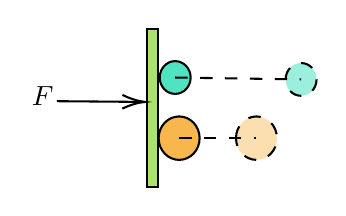
\begin{tikzpicture}[x=0.75pt,y=0.75pt,yscale=-1,xscale=1]
%uncomment if require: \path (0,107); %set diagram left start at 0, and has height of 107

%Shape: Ellipse [id:dp05133763464123664] 
\draw  [fill={rgb, 255:red, 80; green, 227; blue, 194 }  ,fill opacity=1 ] (261.12,39.52) .. controls (261.12,35.16) and (264.45,31.62) .. (268.56,31.62) .. controls (272.68,31.62) and (276.01,35.16) .. (276.01,39.52) .. controls (276.01,43.88) and (272.68,47.41) .. (268.56,47.41) .. controls (264.45,47.41) and (261.12,43.88) .. (261.12,39.52) -- cycle ;
%Shape: Ellipse [id:dp2579371445950144] 
\draw  [fill={rgb, 255:red, 245; green, 166; blue, 35 }  ,fill opacity=0.81 ] (260.6,68.74) .. controls (260.6,62.95) and (265.02,58.27) .. (270.47,58.27) .. controls (275.92,58.27) and (280.34,62.95) .. (280.34,68.74) .. controls (280.34,74.52) and (275.92,79.2) .. (270.47,79.2) .. controls (265.02,79.2) and (260.6,74.52) .. (260.6,68.74) -- cycle ;
%Shape: Rectangle [id:dp8291838904746966] 
\draw  [fill={rgb, 255:red, 126; green, 211; blue, 33 }  ,fill opacity=0.65 ] (254.93,16) -- (260.13,16) -- (260.13,92.07) -- (254.93,92.07) -- cycle ;
%Straight Lines [id:da4542452042526409] 
\draw    (211.59,50.92) -- (252.07,51.26) ;
\draw [shift={(254.07,51.28)}, rotate = 180.49] [color={rgb, 255:red, 0; green, 0; blue, 0 }  ][line width=0.75]    (10.93,-3.29) .. controls (6.95,-1.4) and (3.31,-0.3) .. (0,0) .. controls (3.31,0.3) and (6.95,1.4) .. (10.93,3.29)   ;
%Shape: Ellipse [id:dp09262310823203379] 
\draw  [fill={rgb, 255:red, 80; green, 227; blue, 194 }  ,fill opacity=0.57 ][dash pattern={on 4.5pt off 4.5pt}] (321.79,40.43) .. controls (321.79,36.07) and (325.12,32.54) .. (329.24,32.54) .. controls (333.35,32.54) and (336.68,36.07) .. (336.68,40.43) .. controls (336.68,44.79) and (333.35,48.33) .. (329.24,48.33) .. controls (325.12,48.33) and (321.79,44.79) .. (321.79,40.43) -- cycle ;
%Shape: Ellipse [id:dp24187484540602877] 
\draw  [fill={rgb, 255:red, 245; green, 166; blue, 35 }  ,fill opacity=0.36 ][dash pattern={on 4.5pt off 4.5pt}] (297.87,68.74) .. controls (297.87,62.95) and (302.29,58.27) .. (307.74,58.27) .. controls (313.19,58.27) and (317.61,62.95) .. (317.61,68.74) .. controls (317.61,74.52) and (313.19,79.2) .. (307.74,79.2) .. controls (302.29,79.2) and (297.87,74.52) .. (297.87,68.74) -- cycle ;
%Straight Lines [id:da6202461239130901] 
\draw  [dash pattern={on 4.5pt off 4.5pt}]  (268.56,39.52) -- (329.24,40.43) ;
%Straight Lines [id:da7900556778658151] 
\draw  [dash pattern={on 4.5pt off 4.5pt}]  (270.47,68.74) -- (307.74,68.74) ;

% Text Node
\draw (198,42.36) node [anchor=north west][inner sep=0.75pt]    {$F$};


\end{tikzpicture}

\end{figure}
\noindent
From this, we can say that there exist some innate property of an object which controls the amount of acceleration, even when same force is applied to different objects. This property is the proportionality constant between force and acceleration.\\ We can relate this to some kind of \textit{inertia} (a fashionable way of saying lethargy). We define the \textit{inertial mass} $m^I$ as:
$$m^I := \frac{|\tvec{F}|}{|\tvec{a}|}$$
The inertial mass is a measure of `heaviness to move'.\\[0.2cm]
Now, let us consider the Coulomb's law and Newton's Gravitational Law parallely:
$$\tvec{F}_e = \frac{1}{4\pi \epsilon_0} \frac{q_1 q_2}{\rcurs^2}\hat{\rcurs} \qquad \tvec{F}_g = G  \frac{m_1 m_2}{\rcurs^2}\hat{\rcurs}$$
Similar to $\tvec{F}_e : \mathrm{\ electrical force}$, we have $\tvec{F}_g :\mathrm{\ gravitaional \ force}$ while $\frac{1}{4\pi\epsilon_0} : \mathrm{\ electrostatic \ coupling \ constant}$ is analogous to $G  : \mathrm{\ gravitational \ coupling \ constant}$.\\[0.2cm]
Then indeed the electrical charge $q_i$ must have the analogous gravitational charge $m_i$. Now, note that the gravitational charge, henceforth denoted by $m^G$ has no apriori relation to the previous inertial mass $m^I$ which came from the second law and was a property of the object itself. \\[0.2cm]
We found an electrostatic analog of the gravitational law. It would have been nice to find some \textit{magnetic analog} too, so that, we can also find a combined `force' thing, similar to the Lorentz force $F = q\qty(\tvec{E}+ \vb{v}\times \vb{B})$\\[0.2cm]
Consider the electric due to a charge $Q$ at a point. Then, the force on a charge $q$ kept at the point is given by:
$$\vb{F} = q\vb{E} = m^{I}\vb{a} \implies \vb{a} = \qty(\frac{q}{m^I})\vb{E}$$
The acceleration depends on the charge-mass ratio. Similarly then in a gravitational field, we can write:
$$\vb{F} = m^{G}\vb{g} = m^{I}\vb{a}\implies \vb{a} = \qty(\frac{m^G}{m^I})\vb{g}$$
Till now we had assumed the equality of the two kind of `masses' and then we found that the acceleration due to gravity was independent of masses, that is, every body has the same acceleration due to gravity. However, when we relax this assumption, we are at a critical stage. 
\subsubsection{E\"otv\"os Experiment}